\documentclass[unicode]{beamer}   %Это нам необходимо для объявления призентации
\usepackage{cmap}
\usepackage[utf8]{inputenc}
\usepackage[T2A]{fontenc}
\usepackage[english,russian]{babel} %локализация и переносы  
\usepackage{amsthm,amsmath,amssymb}
\usetheme{Madrid}
\setbeamercolor{titlelike}{parent=structure,bg=gray,fg = white}
\definecolor{myNewColorA}{RGB}{160,160,160}
\definecolor{myNewColorB}{RGB}{255,255,255}
\definecolor{myNewColorC}{RGB}{160,160,160}
\definecolor{myNewColorD}{RGB}{160,160,160}

\setbeamercolor*{palette primary}{bg=myNewColorA, fg = white}
\setbeamercolor*{palette secondary}{bg=myNewColorB, fg = gray}
\setbeamercolor*{palette tertiary}{bg=myNewColorC, fg = white}
\setbeamercolor*{palette quaternary}{bg=myNewColorD, fg = green}


\title[Дипломная работа]{Улучшение робастности динамической системы в продольном канале управления с применением обратной динамики}
% \subtitle[Краткое название]{Полное название}
\author{А.Е. Пащенко}
\institute[МАИ]{Московский авиационный институт}
\date{}
\logo{
\includegraphics[width = 1cm]{img/Герб.png}}

\begin{document}
\maketitle

\begin{frame}{Цель дипломной работы}
\begin{itemize}
    \item <+-> []
    \item <+-> [] \begin{block}{Задачи}
        \begin{itemize}
        \item Расчет ЛТХ, ВПХ, а также характеристик маневренностик
        \item Синтез системы автоматического управления
        \item Рассмотреть один из основных способов улучшения робастности динамической 
        системы c применением обратной динамики при помощи PI-котроллера.
        \end{itemize}
    \end{block}
\end{itemize}    
\end{frame}
\begin{frame}{Объект исследования}

    \begin{figure}[H]
        \center{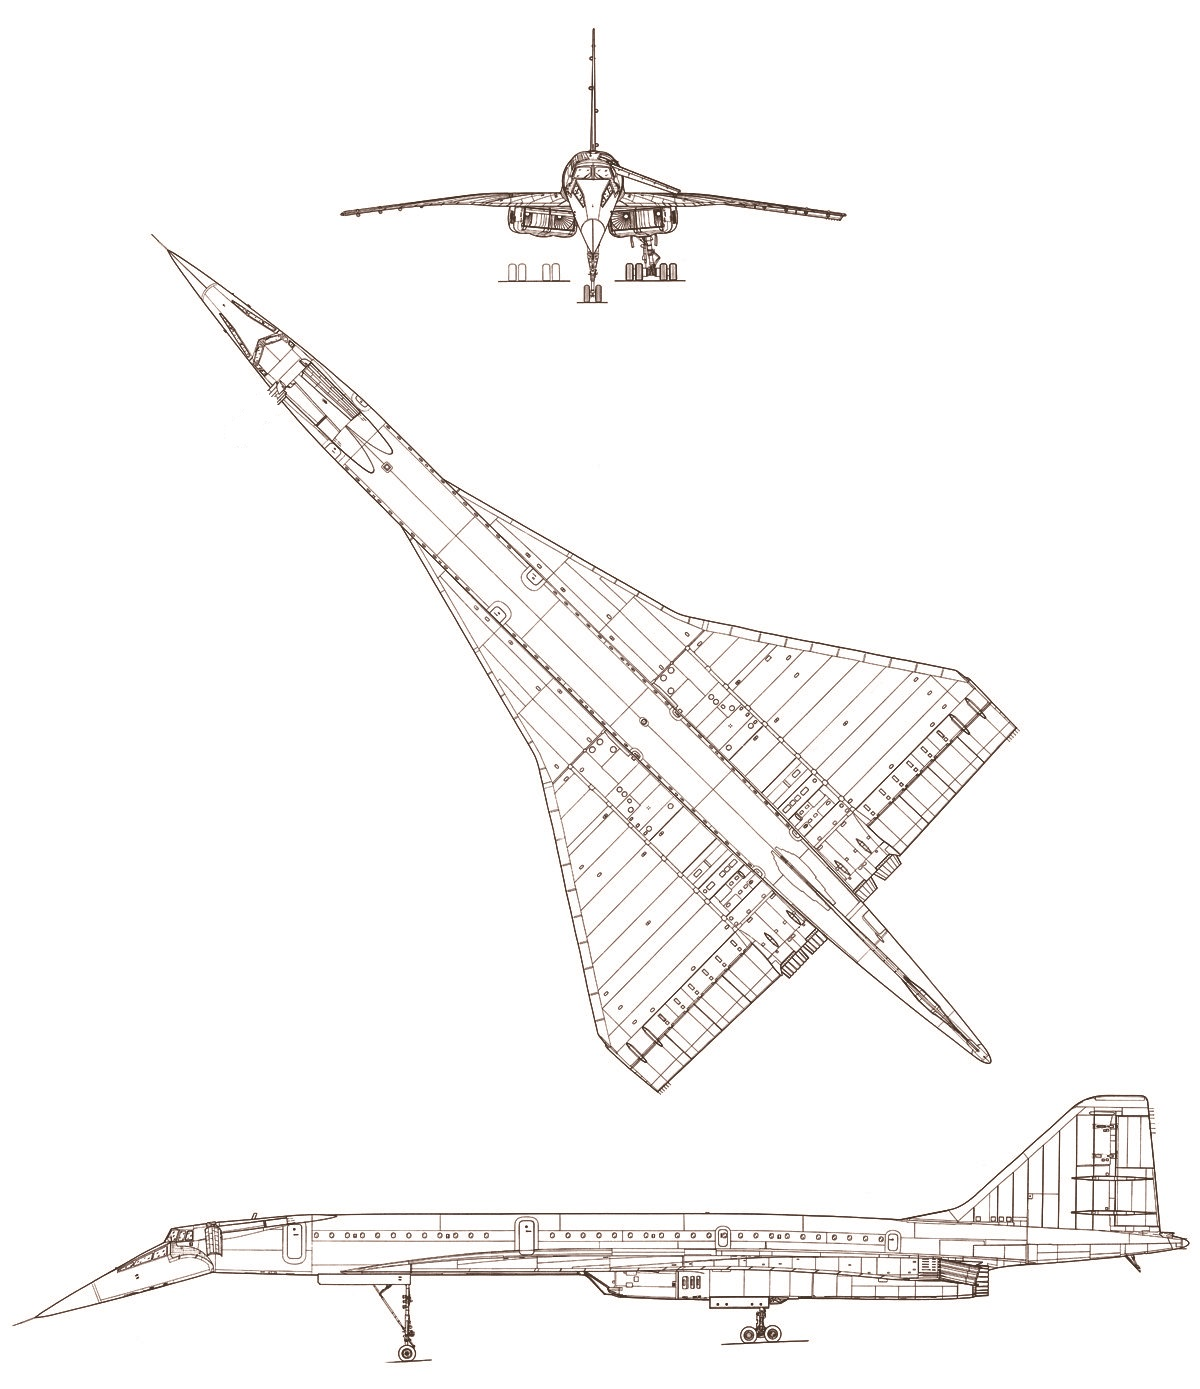
\includegraphics[width=12cm, height = 7cm]{../img/Concorde.jpg}}
        % \caption{Concorde}
        % \label{fig:Concorde}
    \end{figure}

\end{frame}

\begin{frame}{Расчёт ЛТХ}
\begin{block}{В расчёт ЛТХ входит}
   \begin{enumerate}
    \item [] <+->
    \item <+-> Расчёт области возможных полётов
    \item <+-> Расчёт траектории полёта 
    \item <+-> Расчёт транспортных возможностей самолёта
   \end{enumerate}
\end{block}
\end{frame}

\begin{frame}{Расчёт области возможных полётов}

    \begin{block}{Основные ограничения}
        \begin{itemize}
            \item Ограничение по $M_{min \ P}$ 
            \item Ограничение по $M_{max \ P}$
        \end{itemize}
    \end{block}

    \begin{block}{Дополнительные ограничения}
        \begin{itemize}
            \item Ограничение по $C_{y \ \text{доп}}$
            \item Ограничение по $M_\text{пред}$
            \item Ограничение по $q_{maxs}$
        \end{itemize}
    \end{block}

\end{frame}

\begin{frame}{Расчёт области возможных полётов}
    \begin{minipage}[c]{0.55\textwidth}
        \center{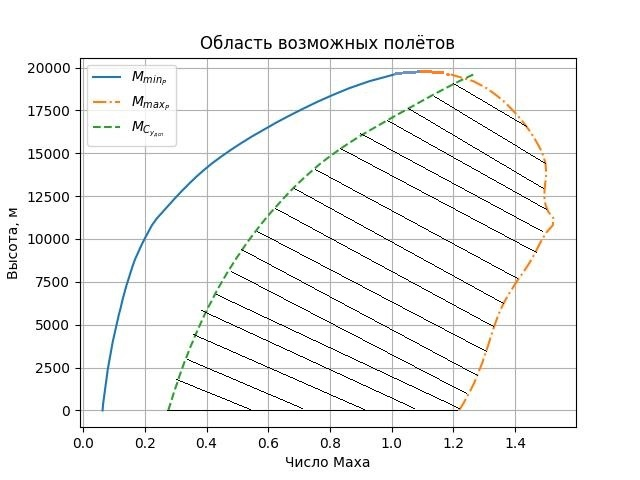
\includegraphics[width=6cm, height = 7cm]{../Оглавление/Part1/figures/Область.jpg}}
    \end{minipage}
    \begin{minipage}[c]{0.4\textwidth}
        \begin{itemize}
            \item <+-> []
            \item <+-> [] \begin{block}{Определение области}
                \begin{itemize}
                    \item $M_{min} = max \{ M_{min \ p}, \ M_{C_{y \ \text{доп}}} \} $
                    \item $M_{max} = min \{ M_{max \ P}, \ M_{\text{пред}}, \ M_{q_{max}} \}$
                \end{itemize}
            \end{block}
        \end{itemize}
    \end{minipage}
\end{frame}

\begin{frame}{Определение теоретического и практического потолка}
    \begin{minipage}[c]{0.45\textwidth}
        \begin{block}{Потолки}
        \begin{itemize}
            \item <+-> []
            \item <+-> [] Расчёт теоретического и практического потолка производится по $V_{y_{max}}$
            \item <+-> [] $H_\text{т} = 19,8$ км 
            \item <+-> [] $H_\text{пр} = 19,5$ км
        \end{itemize}
        \end{block}
    \end{minipage}
    \begin{minipage}[c]{0.45\textwidth}
        \center{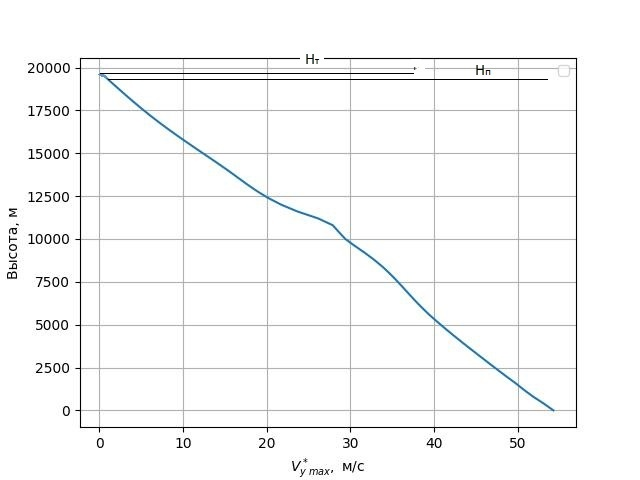
\includegraphics[width=6cm, height = 7cm]{../Оглавление/Part1/figures/Vy(H).jpg}}
    \end{minipage}
\end{frame}

\begin{frame}{Расчёт траектории полёта}
    \begin{block}{Траектория}
    \begin{itemize}
        \item [] <+->
        \item [] <+-> Траеткорию полёта принято разделять на три этапа 
            \begin{itemize}
                \item Набор высоты 
                \item Крейсерский полёт 
                \item Снижение 
            \end{itemize}
    \end{itemize}
    \end{block}
\end{frame}
\begin{frame}{Расчет взлетно-посадочных характеристик самолета}
    \begin{block}{Результаты расчётов}
    \begin{table}
        \begin{tabular}{|c|c|c|c|c|c|}
            \hline
            $V_\text{отр}$, м/с& $L_\text{р}$, м & $L_\text{вд}$, м & $V_\text{кас}$, м/с & $L_\text{проб}$, м & $L_\text{пд}$, м\\ \hline
            88,85& 1125,37 & 1392 & 64,58 & 576 & 1200,78\\ \hline
        \end{tabular}
    \end{table}
\end{block}
\end{frame}

\begin{frame}{Расчёт характеристик манёвренности}
    \begin{block}{Основные положения}
        Для неманёвренного самолёта характеристики предельного правильного виража расcчитываются для высоты $H$= 6км.
        Характеристики маневренности рассчитываются при 50\%-ом выгорании топлива для массы самолета:
        $$\bar{m}_c = 1- 0,5\bar{m}_\text{т}$$
    \end{block}
\end{frame}

\begin{frame}{Расчёт характеристик манёвренности}
    \begin{minipage}[c]{0.45\textwidth}
        \center{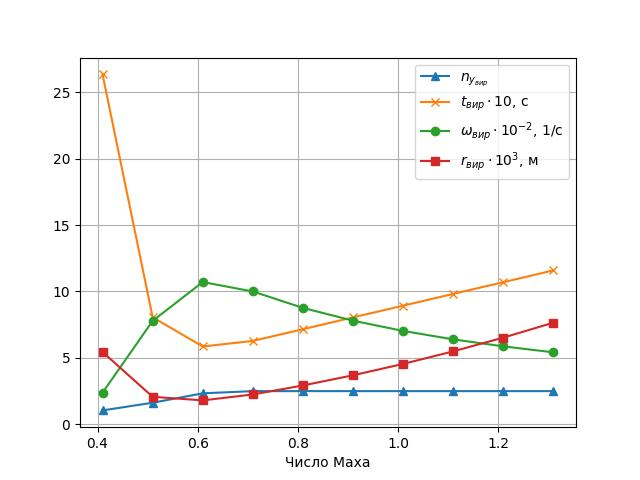
\includegraphics[width=6cm, height = 7cm]{../Оглавление/Part1/figures/РезультатыМаневры.jpg}}
    \end{minipage}  
    \begin{minipage}[c]{0.45\textwidth}
        \center{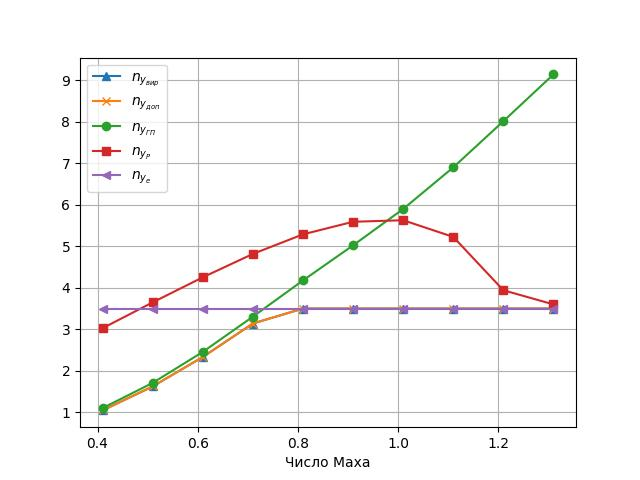
\includegraphics[width=6cm, height = 7cm]{../Оглавление/Part1/figures/РезультатыМаневры2.jpg}}
    \end{minipage}
\end{frame}

\begin{frame}{Благодарность}
\centering
\huge    % Команда меняет шрифт
Спасибо за внимание
\end{frame}

\end{document}
